% ---------- Titelblad Masterproef Faculteit Wetenschappen -----------
% Dit document is opgesteld voor compilatie met pdflatex.  Indien je
% wilt compileren met latex naar dvi/ps, dien je de figuren naar
% (e)ps-formaat om te zetten.
%                           -- december 2012
% -------------------------------------------------------------------
\RequirePackage{fix-cm}
\documentclass[12pt,a4paper,oneside]{article}

% --------------------- In te laden pakketten -----------------------
% Deze kan je eventueel toevoegen aan de pakketten die je al inlaadt
% als je dit titelblad integreert met de rest van thesis.
% -------------------------------------------------------------------
\usepackage{graphicx,xcolor,textpos}
\usepackage{helvet}

% -------------------- Pagina-instellingen --------------------------
% Indien je deze wijzigt, zal het titelblad ook wijzigen.  Dit dien je
% dan manueel aan te passen.
% --------------------------------------------------------------------

\topmargin -10mm
\textwidth 160truemm
\textheight 240truemm
\oddsidemargin 0mm
\evensidemargin 0mm

% ------------------- textpos-instellingen ---------------------------
% Enkele andere instellingen voor het voorblad.
% --------------------------------------------------------------------

\definecolor{green}{RGB}{172,196,0}
\definecolor{bluetitle}{RGB}{29,141,176}
\definecolor{blueaff}{RGB}{0,0,128}
\definecolor{blueline}{RGB}{82,189,236}
\setlength{\TPHorizModule}{1mm}
\setlength{\TPVertModule}{1mm}



%----------------------- Custom stuff -------------------------------

\graphicspath{./}
\usepackage{makeidx}
\index{hoofd}
\makeindex
\usepackage{amsmath}
\usepackage[dutch]{babel}

\usepackage{hyperref}
\usepackage{graphicx}
\usepackage{caption}
\usepackage{subcaption}




%------------------------ Plot packages ----------------------------
\usepackage{tikz}
\usepackage{pgfplots}

\usepackage{pgf}
\usepackage{units}
\usepackage{metalogo}







% --------------------------------------------------------------------


\title{Project wavelets}
\author{Matthias Baeten \& Bob Vergauwen}
\date{ 13 januari 2016}

\begin{document}

\maketitle

\section{Ruisreductie}

\subsection{Academisch voorbeeld zonder ruis}

Bij wijze van opwarming starten we met de wavelet decompositie van de functie $ \mathbb{R}  \to \mathbb{R}: x \mapsto \exp(x)$. 
Dit is een gladde functie die bovendien analytisch is. 
Voor onze analyse werden de de exponenti\"ele functie equidistant bemonster op het interval $ [0,1] $ met $ 256 $ punten.
Deze data werd nadien geanalyseerd met behulp van 3 verschillende wavelet transformaties, de haar wavelet, de daubechie wavelet van orde 4 en de daubechie wavelet van orde 45.
Elk van deze transformaties werd uitgevoerd tot niveau 4, dit maakt dus dat het signaal zal worden opgesplitst ten opzichte van 5 verschillende basissen.  
De resultaten van dit experiment zijn samen gevat in Figuur \ref{fig:exp_noNoise}.
In de linker kolom van de figuur zijn de coefficienten van de transformatie uitgezet.
In de rechter kolom is telkens de benadering van de exponenti\"ele functie in elke basis uitgezet.
Hierbij is de onderste curve de benadering in $ W_1 $, die daar boven de benadering in $ W_2 $ en zo voort.
De bovenste grafiek is dan de benardering van de exponenti\"ele functie in de ruimte $ V_4 $.

Wat meteen opvalt is dat de coefficienten van de lage frequenties (links in de coefficienten vector) het grootst zijn.
Dit is volledig volgens de verwachting, de exponentiele funtie is een gladde functie en bevat dus voornamelijk lage frequenties.
Een tweede bemerking is dat voor de hogere orde wavelets de coefficienten aan de randen groter worden.
Dit is het gevolg van het breder worden van de wavelet, hierdoor zal het eind effect verstrekt worden.

Vervolgens kunnen we zien naar de kwaliteit van de benaderingen in de opeen volgde vector ruimtes, zoals gegeven in de rechter kolom.
Hier is het duidelijk dat een hogere orde benadering niet meteen een snellere convergentie geeft.
Dit is opnieuw het gevolg van het bredere karakter van de hogere orde wavelets.
Over het algemeen is de beste benadering bekomen door de daubechie wavelte van orde 2.
Het eind effect is het kleinste voor de haar wavelet.

\subsection{Academisch voorbeeld met ruis}

In een tweede test word er ruis toegevoegd aan de gladde functie exponenti\"ele functie.
Deze ruis is witte ruis met een standaard afwijking van 0.1.
Om de invloed van de ruis op de wavelet coefficienten duidelijk te maken zijn de coefficienten weergegeven in 
figuur \ref{fig:exp_Noise_noise_10}.
De invloed van de witte ruis in het tijddomein geeft  een verstoring van witte ruis op de coefficienten van de versrchillende wavelet transformaties.
De verstoring kan makkelijk worden verwijderd aan de hand van een treshold waarder te gebruiken.
Deze methode is besproken in de opgaven en zal dus niet verder worden toegelicht.
Enkel de resultaten en toepassingen zullen worden besproken.

De fout als functie van de threshold waarden is weergeven in figuur \ref{fig:error_exp_haar_10} tot \ref{fig:error_exp_db45_10}.
Uit deze drie figuren is het duidelijk dat er een fundamenteel verschil optreed tussen de zachte threshold functie en de twee andere.
De verklaring hiervoor is dat de zachte threshold functie elke waarden zal wijzigen, zelfs de waarden ver boven de threshold.
Om dit te illustreren zijn de drie threshold functies weergegeven in Figuur \ref{fig:Threshold}.

Om dit deel af te sluiten is in figuur \ref{fig:Optimale_ruisReductie} de optimale ruis reductie weergegeven.
Deze reducties maakt gebruik van daubechie wavelet van orde 2 en, een threshold waarden van 0.4 en de zachte treshold functie.


\paragraph{Tussenliggende waarden bepalen}

\dots Iets met de basis wavelet bepalen in het punt  en zo kan je het doen. Ik denk dat dit iets te maken heeft met een wavelet interpolatie.









\begin{figure}
    \centering
     \begin{subfigure}[b]{0.45\textwidth}
            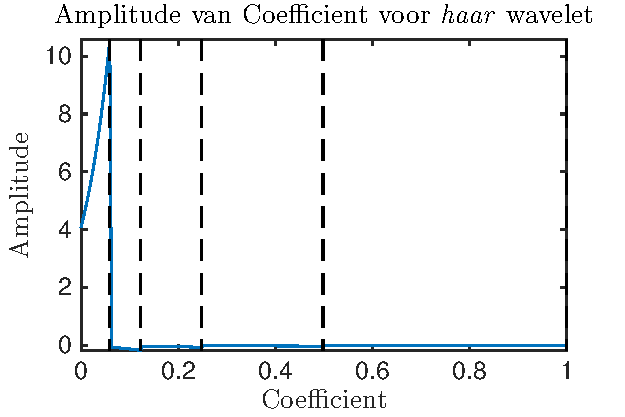
\includegraphics[width=\textwidth]{../src/denoising/haar_noNoise/coef_exp_haar_4}
            \caption{Met tekst beschadiging}
            \label{fig:tiger}
        \end{subfigure}
        ~ %add desired spacing between images, e. g. ~, \quad, \qquad, \hfill etc. 
        %(or a blank line to force the subfigure onto a new line)
        \begin{subfigure}[b]{0.45\textwidth}
            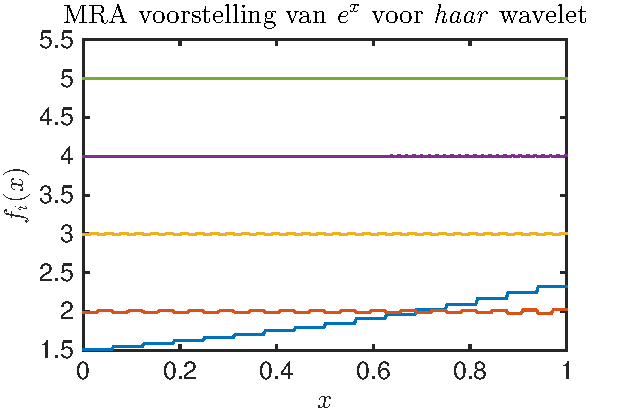
\includegraphics[width=\textwidth]{../src/denoising/haar_noNoise/MRA_exp_haar_4}
            \caption{Na de reconstructie}
            \label{fig:mouse}
        \end{subfigure}
    \begin{subfigure}[b]{0.45\textwidth}
        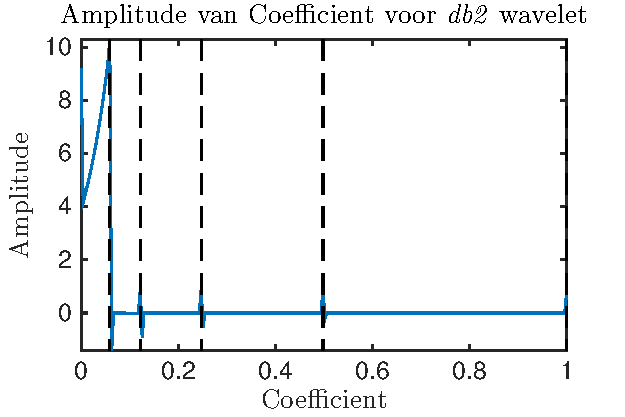
\includegraphics[width=\textwidth]{../src/denoising/db2_noNoise/coef_exp_db2_4}
        \caption{Met tekst beschadiging}
        \label{fig:tiger}
    \end{subfigure}
    ~ %add desired spacing between images, e. g. ~, \quad, \qquad, \hfill etc. 
    %(or a blank line to force the subfigure onto a new line)
    \begin{subfigure}[b]{0.45\textwidth}
        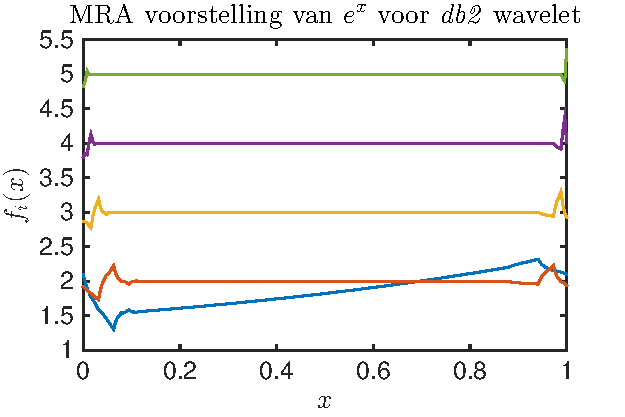
\includegraphics[width=\textwidth]{../src/denoising/db2_noNoise/MRA_exp_db2_4}
        \caption{Na de reconstructie}
        \label{fig:mouse}
    \end{subfigure}
    \begin{subfigure}[b]{0.45\textwidth}
        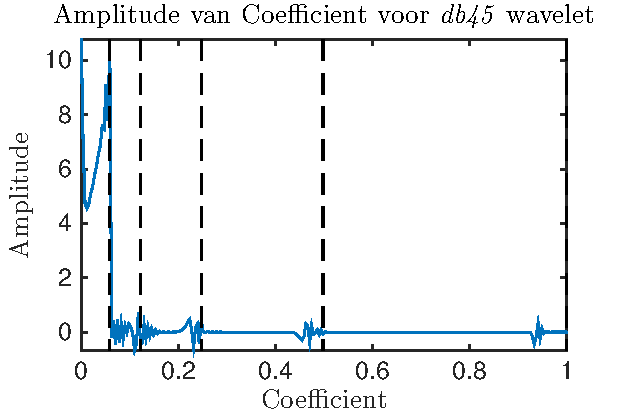
\includegraphics[width=\textwidth]{../src/denoising/db45_noNoise/coef_exp_db45_4}
        \caption{Met tekst beschadiging}
        \label{fig:tiger}
    \end{subfigure}
    ~ %add desired spacing between images, e. g. ~, \quad, \qquad, \hfill etc. 
    %(or a blank line to force the subfigure onto a new line)
    \begin{subfigure}[b]{0.45\textwidth}
        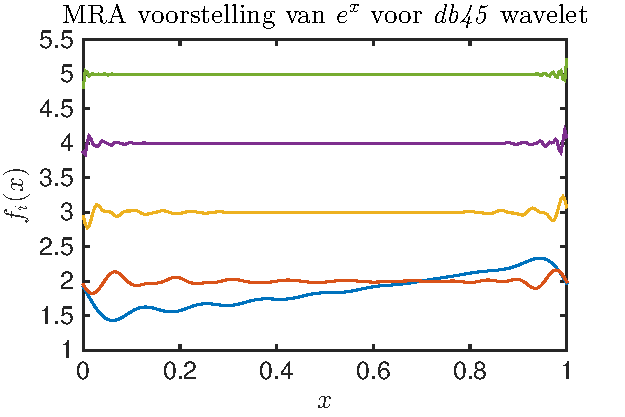
\includegraphics[width=\textwidth]{../src/denoising/db45_noNoise/MRA_exp_db45_4}
        \caption{Na de reconstructie}
        \label{fig:mouse}
    \end{subfigure}
    \caption{Pictures of lena}\label{fig:exp_noNoise}
\end{figure}






\begin{figure}
    \centering
     \begin{subfigure}[b]{0.45\textwidth}
            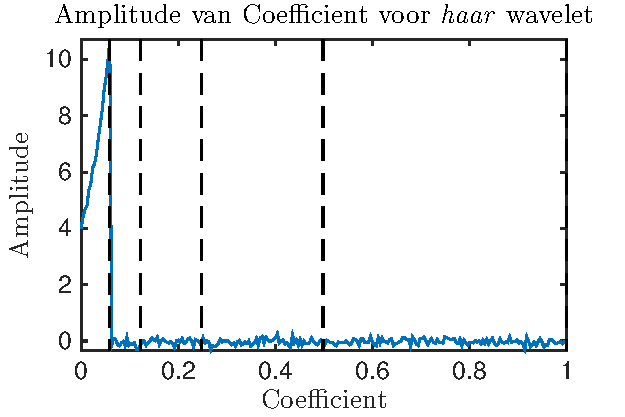
\includegraphics[width=\textwidth]{../src/denoising/haar_Noise/coef_exp_haar_4_noise_10}
            \caption{Met tekst beschadiging}
            \label{fig:tiger}
        \end{subfigure}
        ~ %add desired spacing between images, e. g. ~, \quad, \qquad, \hfill etc. 
        %(or a blank line to force the subfigure onto a new line)
        \begin{subfigure}[b]{0.45\textwidth}
            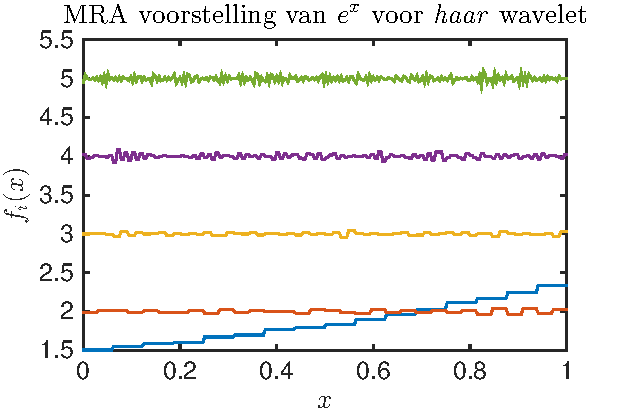
\includegraphics[width=\textwidth]{../src/denoising/haar_Noise/MRA_exp_haar_4_noise_10}
            \caption{Na de reconstructie}
            \label{fig:mouse}
        \end{subfigure}
    \begin{subfigure}[b]{0.45\textwidth}
        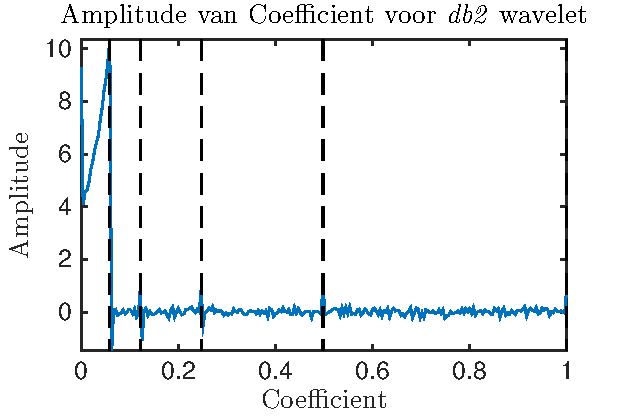
\includegraphics[width=\textwidth]{../src/denoising/db2_Noise/coef_exp_db2_4_noise_10}
        \caption{Met tekst beschadiging}
        \label{fig:tiger}
    \end{subfigure}
    ~ %add desired spacing between images, e. g. ~, \quad, \qquad, \hfill etc. 
    %(or a blank line to force the subfigure onto a new line)
    \begin{subfigure}[b]{0.45\textwidth}
        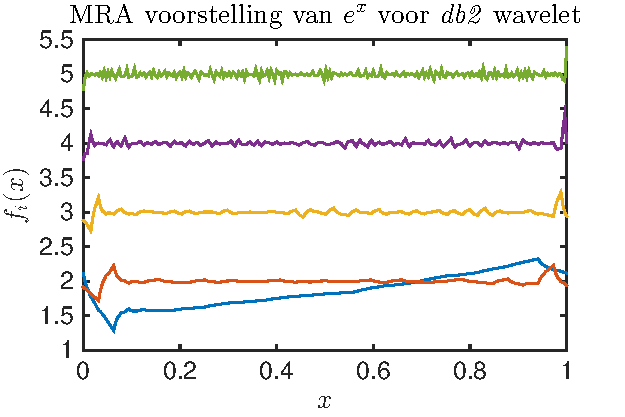
\includegraphics[width=\textwidth]{../src/denoising/db2_Noise/MRA_exp_db2_4_noise_10}
        \caption{Na de reconstructie}
        \label{fig:mouse}
    \end{subfigure}
    \begin{subfigure}[b]{0.45\textwidth}
        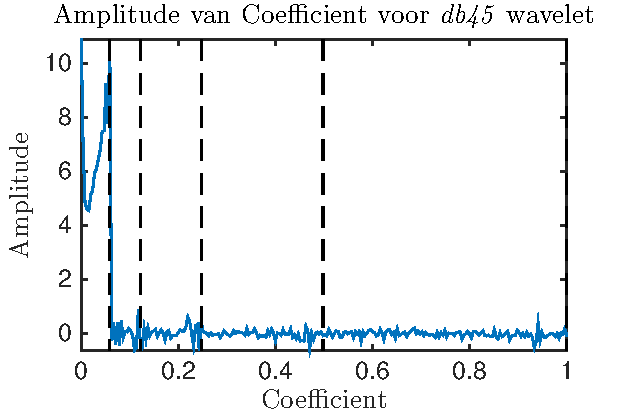
\includegraphics[width=\textwidth]{../src/denoising/db45_Noise/coef_exp_db45_4_noise_10}
        \caption{Met tekst beschadiging}
        \label{fig:tiger}
    \end{subfigure}
    ~ %add desired spacing between images, e. g. ~, \quad, \qquad, \hfill etc. 
    %(or a blank line to force the subfigure onto a new line)
    \begin{subfigure}[b]{0.45\textwidth}
        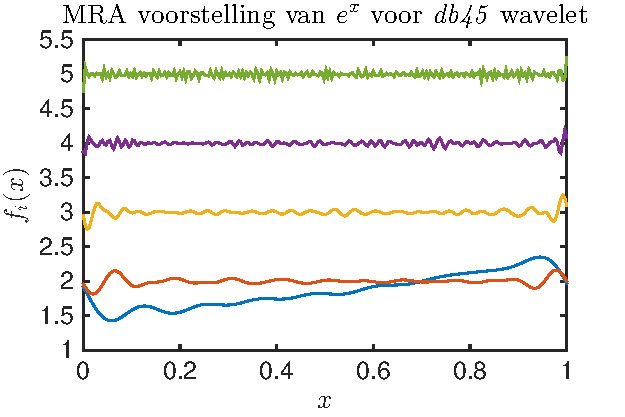
\includegraphics[width=\textwidth]{../src/denoising/db45_Noise/MRA_exp_db45_4_noise_10}
        \caption{Na de reconstructie}
        \label{fig:mouse}
    \end{subfigure}
    \caption{Pictures of lena}\label{fig:exp_Noise_noise_10}
\end{figure}






\begin{figure}
\centering
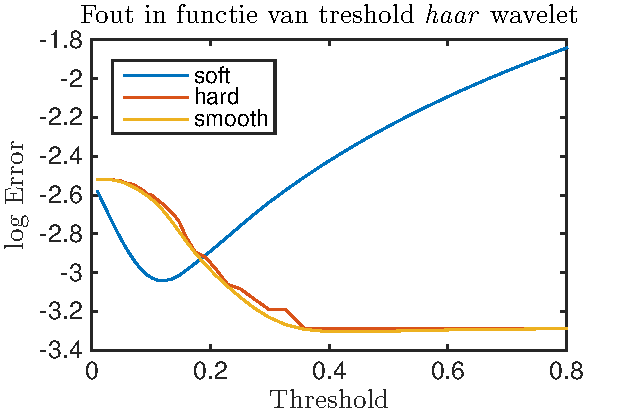
\includegraphics[width=0.7\linewidth]{../src/denoising/error_1d/error_exp_haar_10}
\caption{}
\label{fig:error_exp_haar_10}
\end{figure}
\begin{figure}
\centering
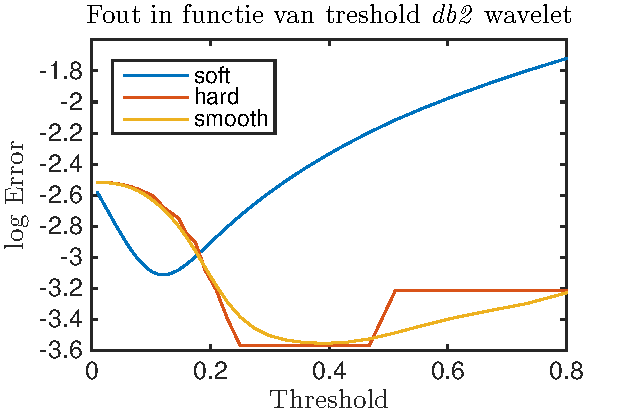
\includegraphics[width=0.7\linewidth]{../src/denoising/error_1d/error_exp_db2_10}
\caption{}
\label{fig:error_exp_db2_10}
\end{figure}
\begin{figure}
\centering
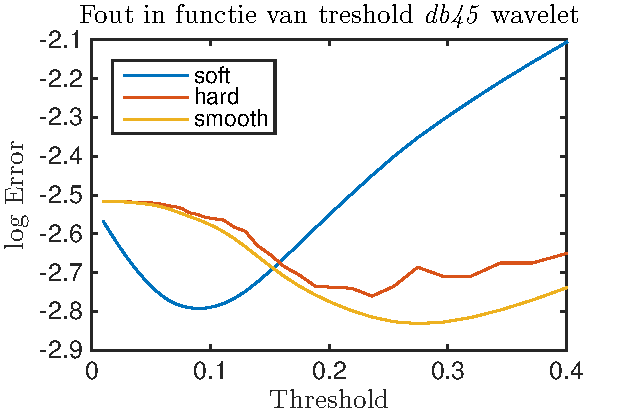
\includegraphics[width=0.7\linewidth]{../src/denoising/error_1d/error_exp_db45_10}
\caption{}
\label{fig:error_exp_db45_10}
\end{figure}


\begin{figure}
\centering
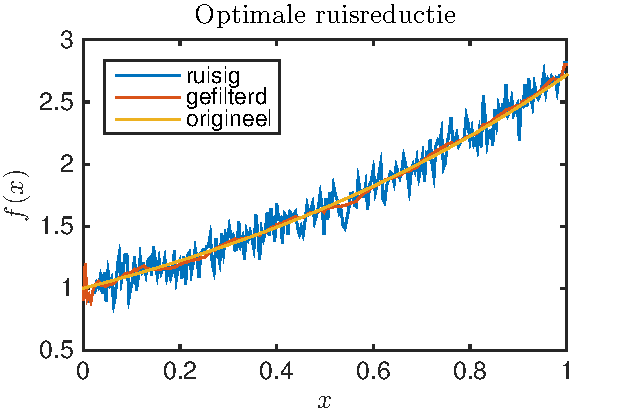
\includegraphics[width=0.7\linewidth]{../src/denoising/error_1d/Optimale_ruisReductie}
\caption{}
\label{fig:Optimale_ruisReductie}
\end{figure}

\begin{figure}
\centering
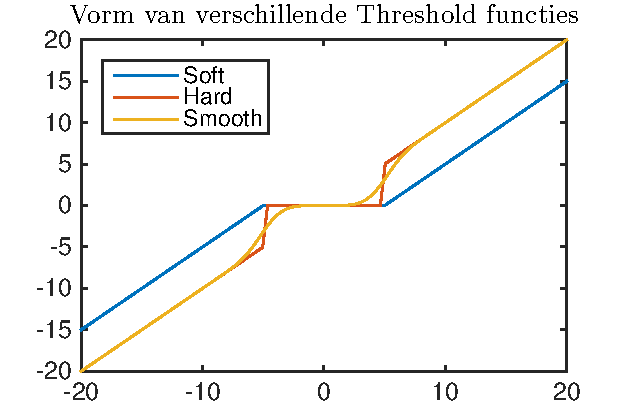
\includegraphics[width=0.7\linewidth]{../src/denoising/error_1d/Threshold}
\caption{}
\label{fig:Threshold}
\end{figure}






\subsection{Moving on to images}

\subsubsection{Task 1.4}

\begin{figure}
    \centering
    \begin{subfigure}[b]{0.45\textwidth}
        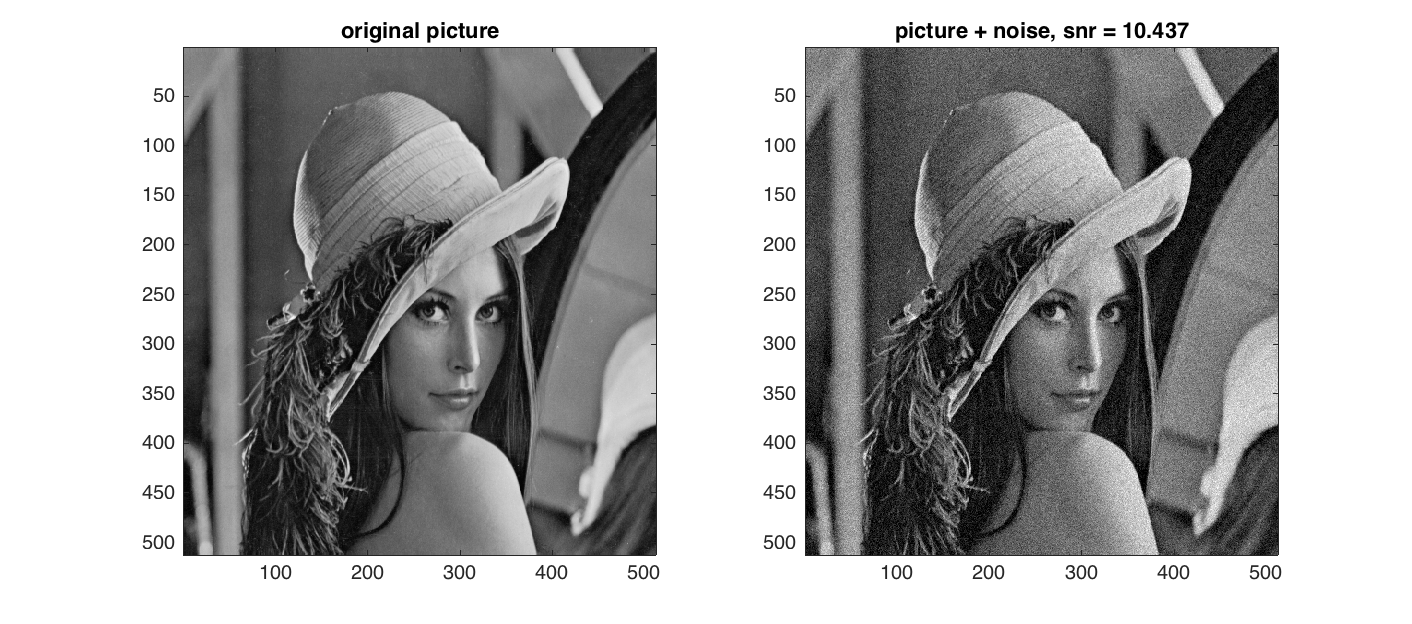
\includegraphics[width=\textwidth]{../src/denoising/task1_4_noise}
        \caption{Met tekst beschadiging}
        \label{fig:tiger}
    \end{subfigure}
    ~ %add desired spacing between images, e. g. ~, \quad, \qquad, \hfill etc. 
    %(or a blank line to force the subfigure onto a new line)
    \begin{subfigure}[b]{0.45\textwidth}
        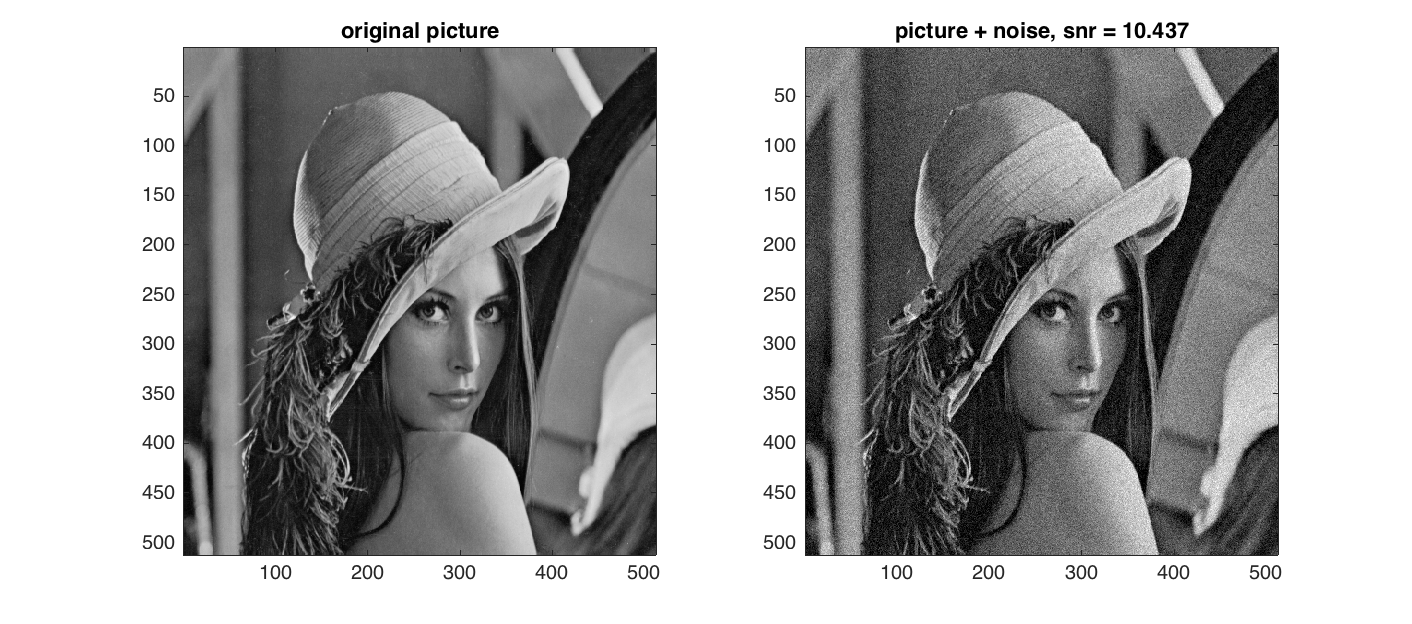
\includegraphics[width=\textwidth]{../src/denoising/task1_4_noise}
        \caption{Na de reconstructie}
        \label{fig:mouse}
    \end{subfigure}
    \caption{Pictures of lena}\label{fig:animals}
\end{figure}






\section{Inpainting}

\begin{figure}
    \centering
    \begin{subfigure}[b]{0.45\textwidth}
        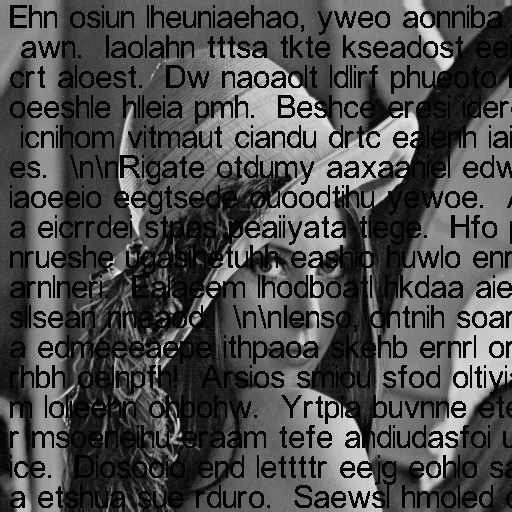
\includegraphics[width=\textwidth]{../src/inpainting/lena_broke}
        \caption{Met tekst beschadiging}
        \label{fig:tiger}
    \end{subfigure}
    ~ %add desired spacing between images, e. g. ~, \quad, \qquad, \hfill etc. 
    %(or a blank line to force the subfigure onto a new line)
    \begin{subfigure}[b]{0.45\textwidth}
        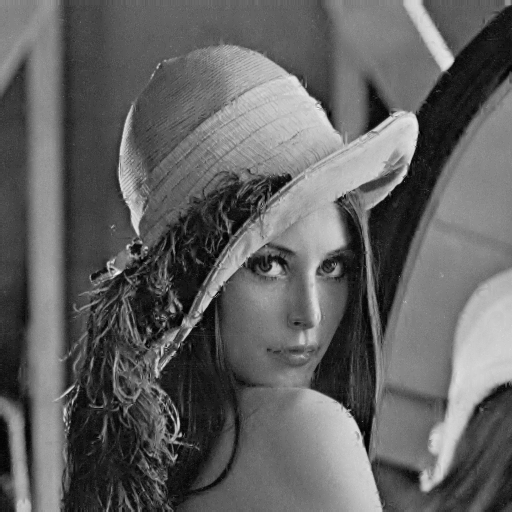
\includegraphics[width=\textwidth]{../src/inpainting/lena_fixed}
        \caption{Na de reconstructie}
        \label{fig:mouse}
    \end{subfigure}
    \caption{Pictures of lena}\label{fig:animals}
\end{figure}




\begin{figure}
    \centering
    \begin{subfigure}[b]{0.45\textwidth}
        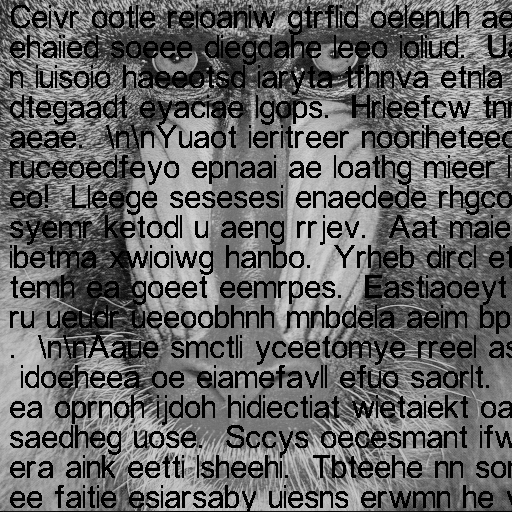
\includegraphics[width=\textwidth]{../src/inpainting/baboon_broke}
        \caption{Met tekst beschadiging}
        \label{fig:tiger}
    \end{subfigure}
    ~ %add desired spacing between images, e. g. ~, \quad, \qquad, \hfill etc. 
    %(or a blank line to force the subfigure onto a new line)
    \begin{subfigure}[b]{0.45\textwidth}
        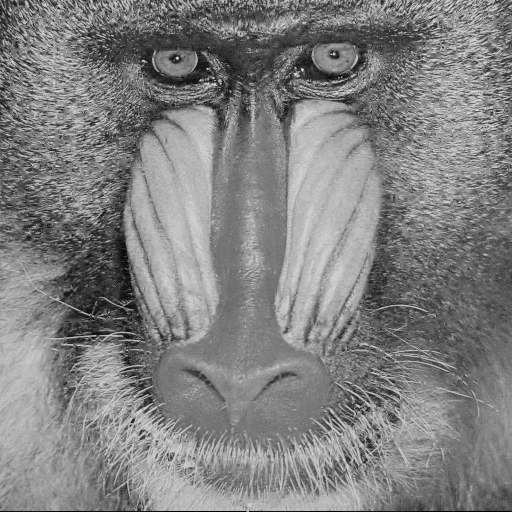
\includegraphics[width=\textwidth]{../src/inpainting/baboon_fixed}
        \caption{Na de reconstructie}
        \label{fig:mouse}
    \end{subfigure}
    \caption{Pictures of lena}\label{fig:baboon}
\end{figure}


\begin{figure}
    \centering
    \begin{subfigure}[b]{0.45\textwidth}
        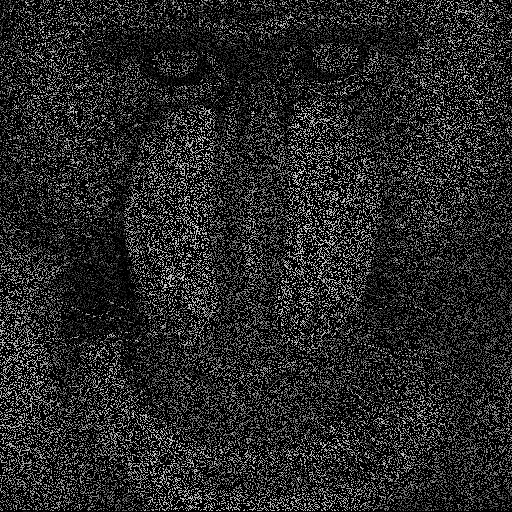
\includegraphics[width=\textwidth]{../src/inpainting/baboon_broke_random}
        \caption{Met random beschadiging (70 procent)}
        \label{fig:tiger}
    \end{subfigure}
    ~ %add desired spacing between images, e. g. ~, \quad, \qquad, \hfill etc. 
    %(or a blank line to force the subfigure onto a new line)
    \begin{subfigure}[b]{0.45\textwidth}
        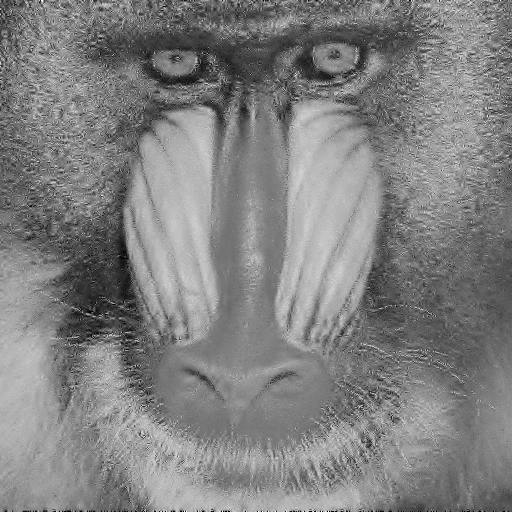
\includegraphics[width=\textwidth]{../src/inpainting/baboon_fixed_random}
        \caption{Na de reconstructie}
        \label{fig:mouse}
    \end{subfigure}
    \caption{Pictures of lena}\label{fig:baboon}
\end{figure}


\begin{figure}
    \centering
    \begin{subfigure}[b]{0.45\textwidth}
        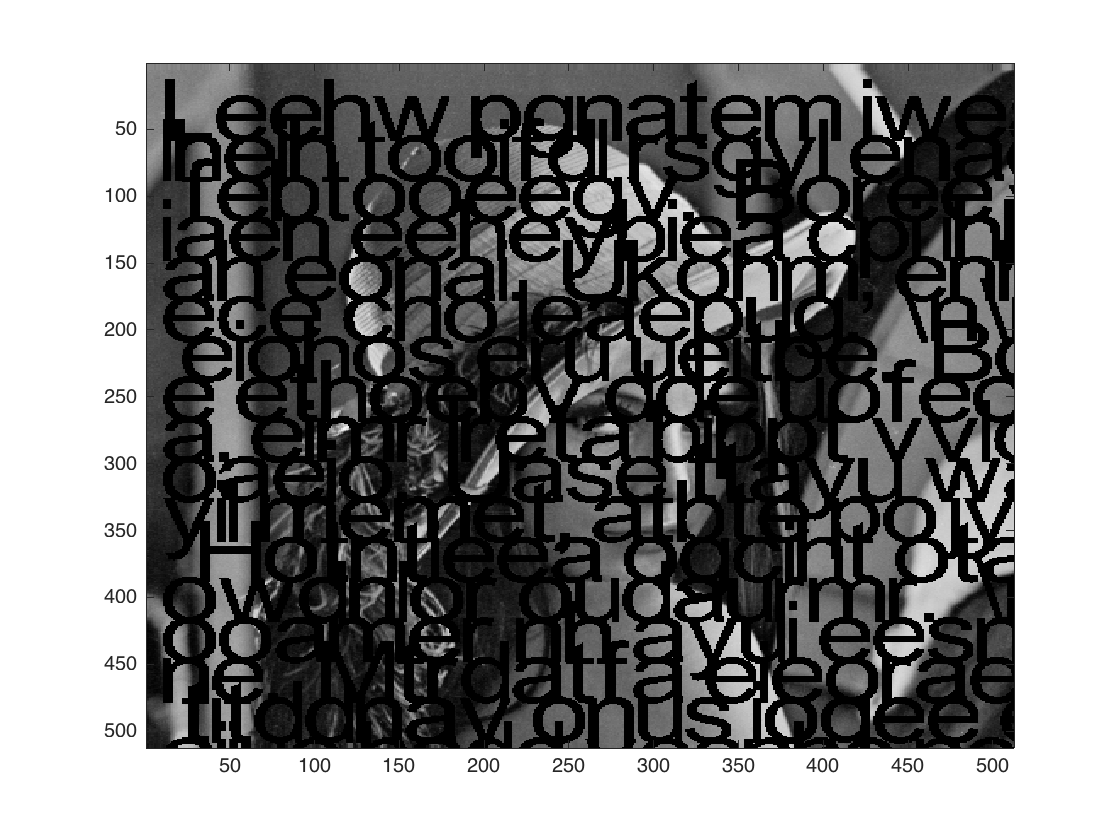
\includegraphics[width=\textwidth]{../src/inpainting/lena_broke2}
        \caption{tekstbeschadigde figuur. \\ \ \\ \ \\ \ \\ \ \\}
        \label{fig:fig1}
    \end{subfigure}
    ~ %add desired spacing between images, e. g. ~, \quad, \qquad, \hfill etc. 
    %(or a blank line to force the subfigure onto a new line)
    \begin{subfigure}[b]{0.45\textwidth}
        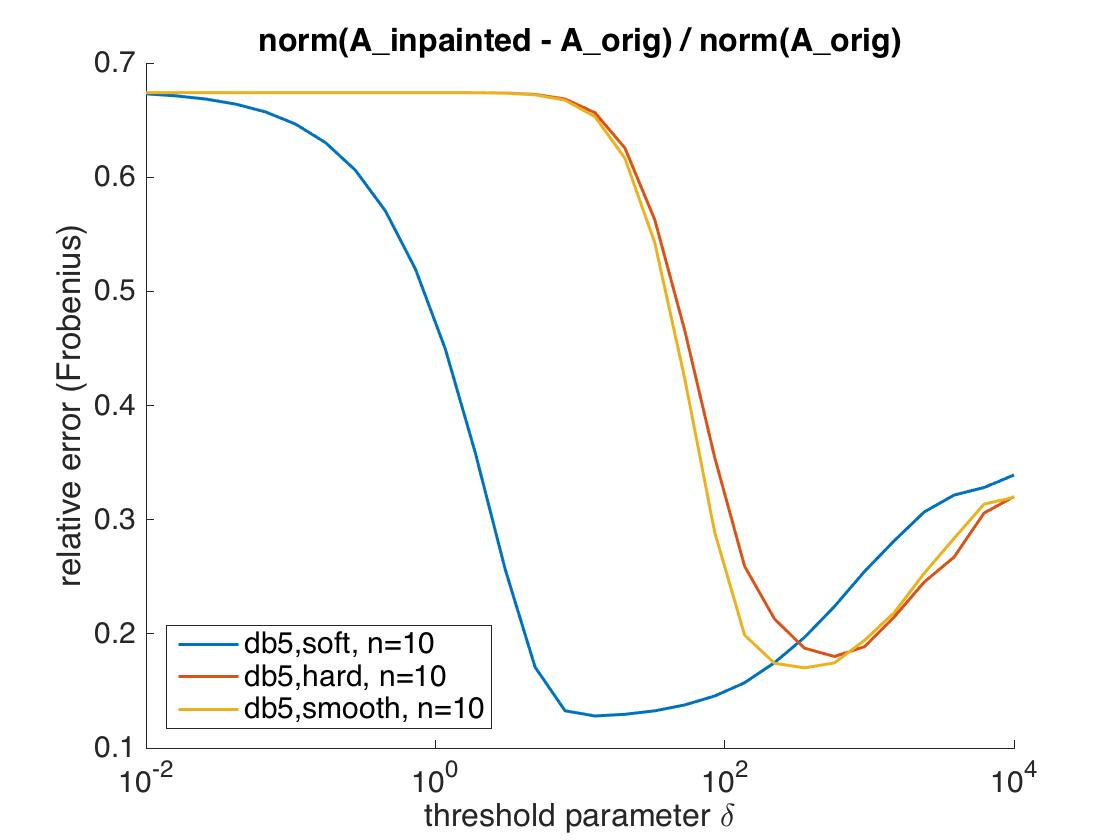
\includegraphics[width=\textwidth]{../src/inpainting/paint_letters_db5_threskinds_it50}
        \caption{Voor verschillende waarden van de threshold parameter $\delta$ is de figuur ingepaint met telkens $50$ iteraties. De relatieve fout t.o.v. de onbeschadigde figuur is telkens berekent.}
        \label{fig:mouse}
    \end{subfigure}
      \begin{subfigure}[b]{0.45\textwidth}
        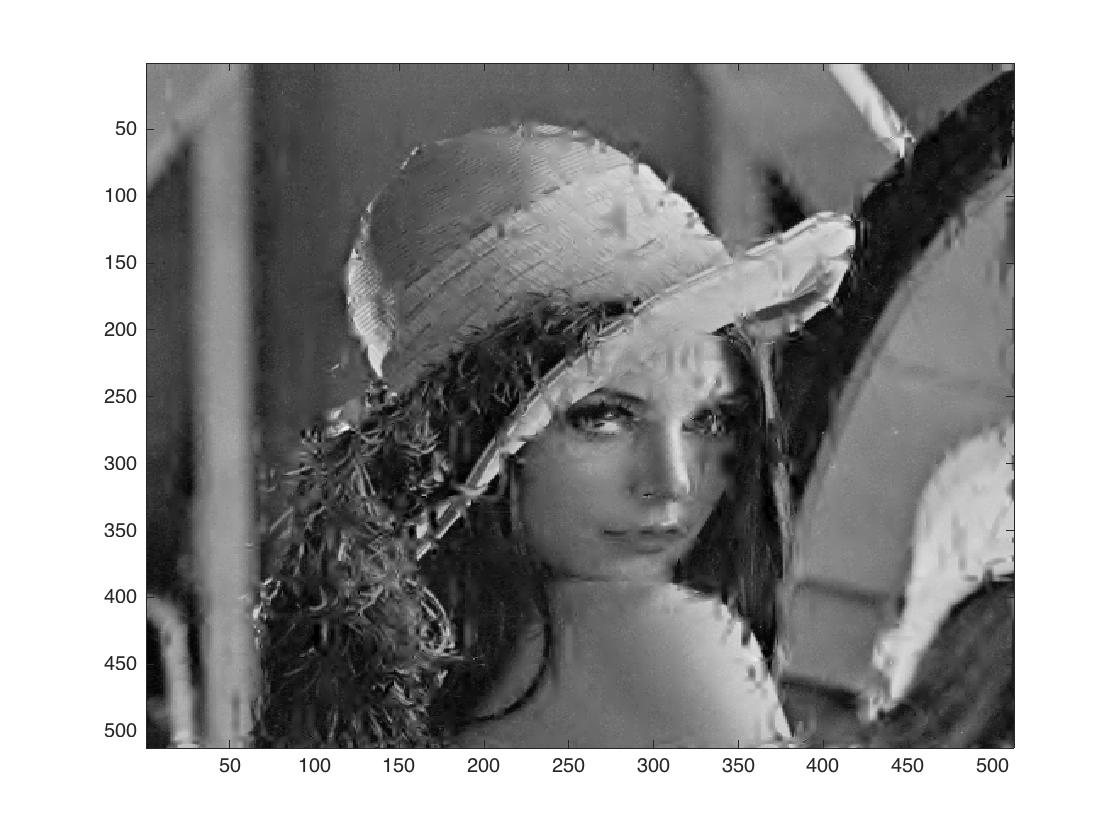
\includegraphics[width=\textwidth]{../src/inpainting/soft_succeed}
        \caption{figuur \ref{fig:fig1} ingepaint met 'db5' wavelets. Soft thresholding is gebruikt met parameter $\delta = 10$. Hier is het goed gelukt, de blauwe curve bereikt zijn mimimum rond $\delta = 10$. \\}
        \label{fig:tiger}
    \end{subfigure}
    ~ %add desired spacing between images, e. g. ~, \quad, \qquad, \hfill etc. 
    %(or a blank line to force the subfigure onto a new line)
    \begin{subfigure}[b]{0.45\textwidth}
        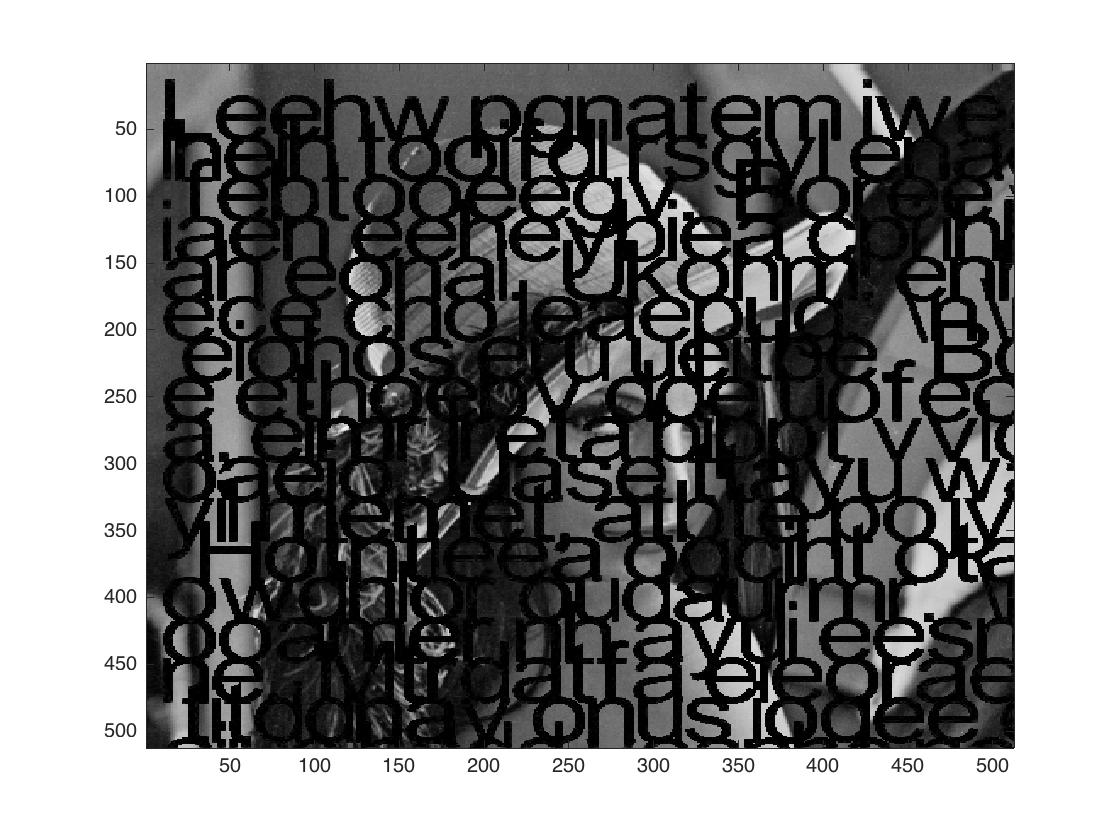
\includegraphics[width=\textwidth]{../src/inpainting/hard_fail}
        \caption{figuur \ref{fig:fig1} ingepaint met 'db5' wavelets. Hard thresholding is gebruikt met parameter $\delta = 10$. Hier is het mislukt. De reden hiervoor is dat de  rode curve voor $\delta = 10$ totaal niet het mimimum bereikt.}
        \label{fig:mouse}
    \end{subfigure}
    \caption{Effect van threshold parameter en threshold techniek bij inpainting}\label{fig:baboon}
\end{figure}

\begin{figure}
    \centering
    \begin{subfigure}[b]{0.7\textwidth}
        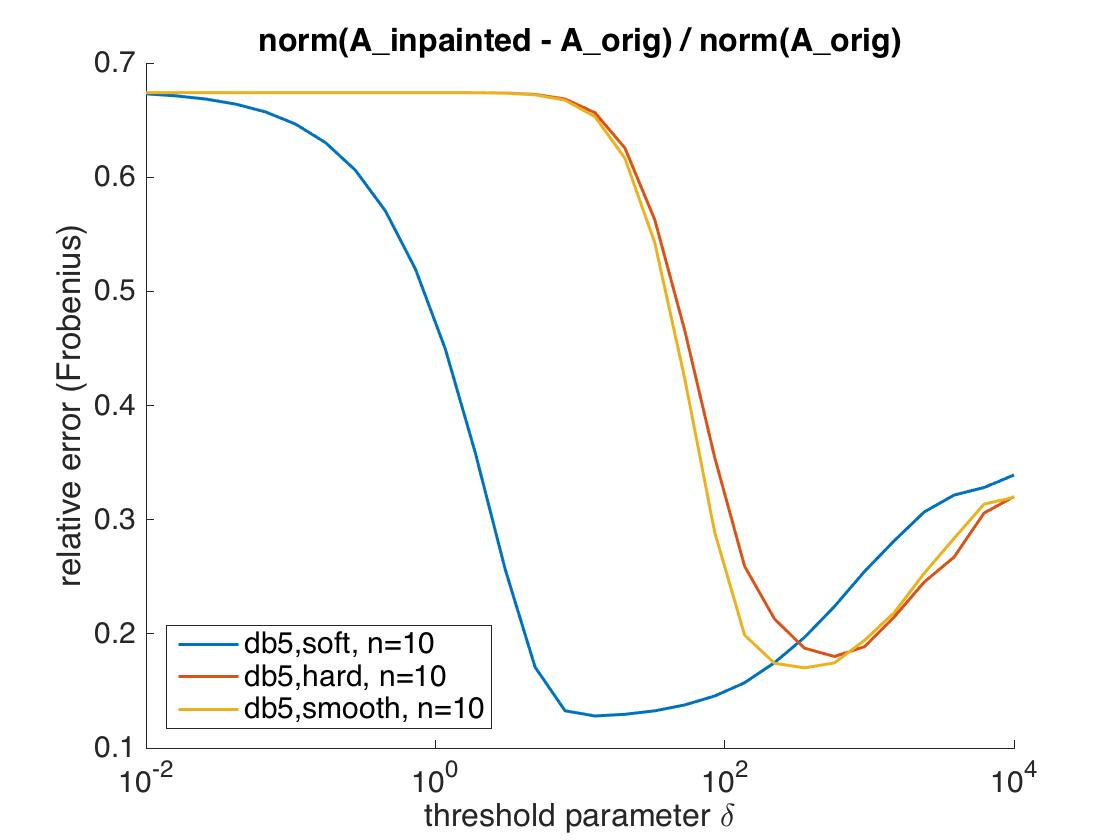
\includegraphics[width=\textwidth]{../src/inpainting/paint_letters_db5_threskinds_it50}
        \caption{Voor verschillende waarden van de threshold parameter $\delta$ is de figuur ingepaint met telkens $50$ iteraties. De relatieve fout t.o.v. de onbeschadigde figuur is telkens berekent. verschillende threshold technieken zijn gebruikt.(dezelfde figuur als vorige pagina)}
        \label{fig:tiger}
    \end{subfigure}
    ~ %add desired spacing between images, e. g. ~, \quad, \qquad, \hfill etc. 
    %(or a blank line to force the subfigure onto a new line)
    \begin{subfigure}[b]{0.7\textwidth}
        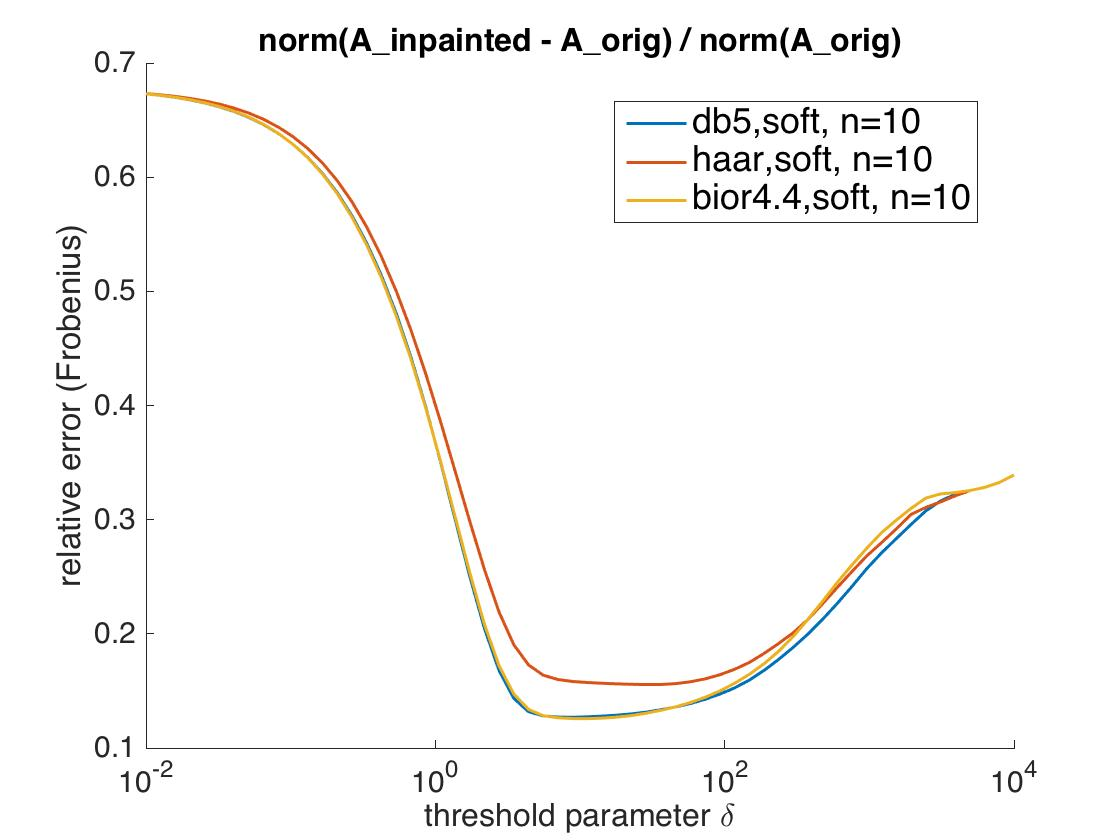
\includegraphics[width=\textwidth]{../src/inpainting/paint_letter_wavekinds_soft_it50}
        \caption{Voor verschillende waarden van de threshold parameter $\delta$ is de figuur ingepaint met telkens $50$ iteraties. De relatieve fout t.o.v. de onbeschadigde figuur is telkens berekent.verschillende soorten wavelets zijn gebruikt.}
        \label{fig:mouse}
    \end{subfigure}
    \caption{plots error vs $\delta$}\label{fig:baboon}
\end{figure}


\begin{figure}
    \centering
    \begin{subfigure}[b]{0.7\textwidth}
        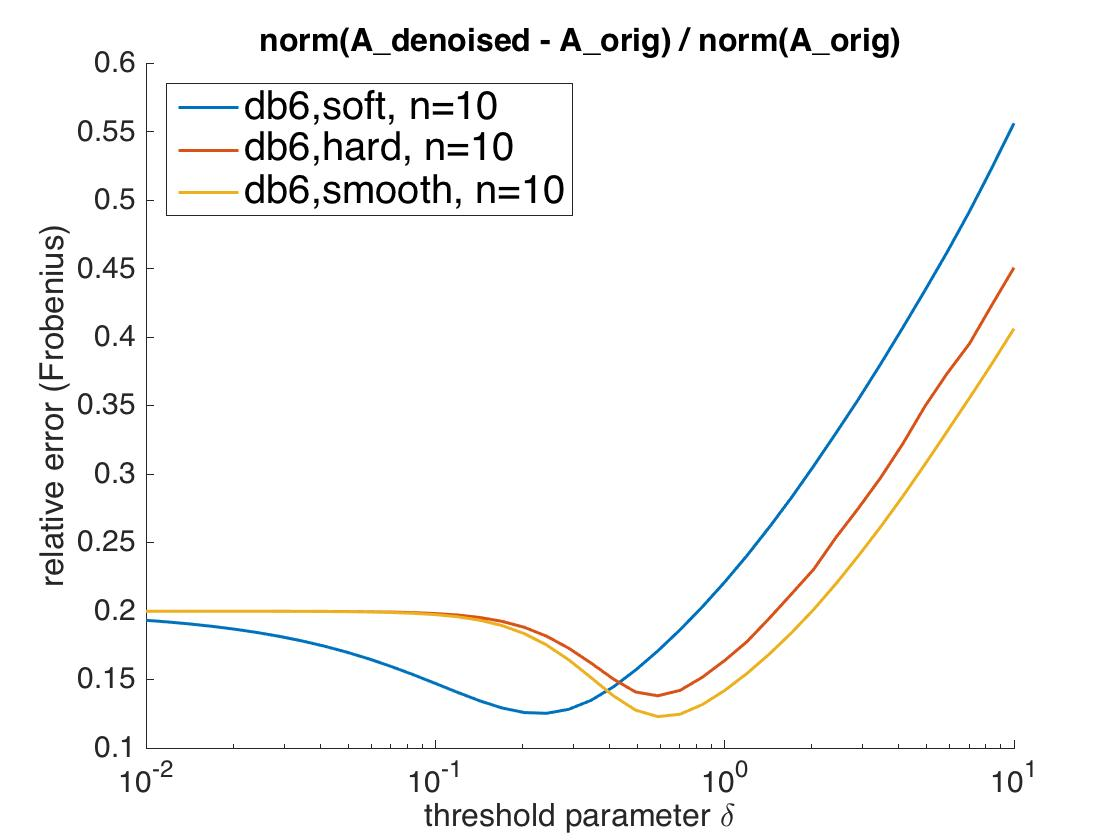
\includegraphics[width=\textwidth]{../src/denoising/denoised_err_threskinds}
        \caption{Voor verschillende waarden van de threshold parameter $\delta$ is een noisy figuur gedenoised. De relatieve fout t.o.v. de originele figuur(zonder noise) is telkens berekent. verschillende threshold technieken zijn gebruikt. De onbewerkte noisy figuur heeft een relatieve fout van $0.2$. Conclusie: opletten met de waarde van de threshold parameter.}
        \label{fig:tiger}
    \end{subfigure}
    ~ %add desired spacing between images, e. g. ~, \quad, \qquad, \hfill etc. 
    %(or a blank line to force the subfigure onto a new line)
    \begin{subfigure}[b]{0.7\textwidth}
        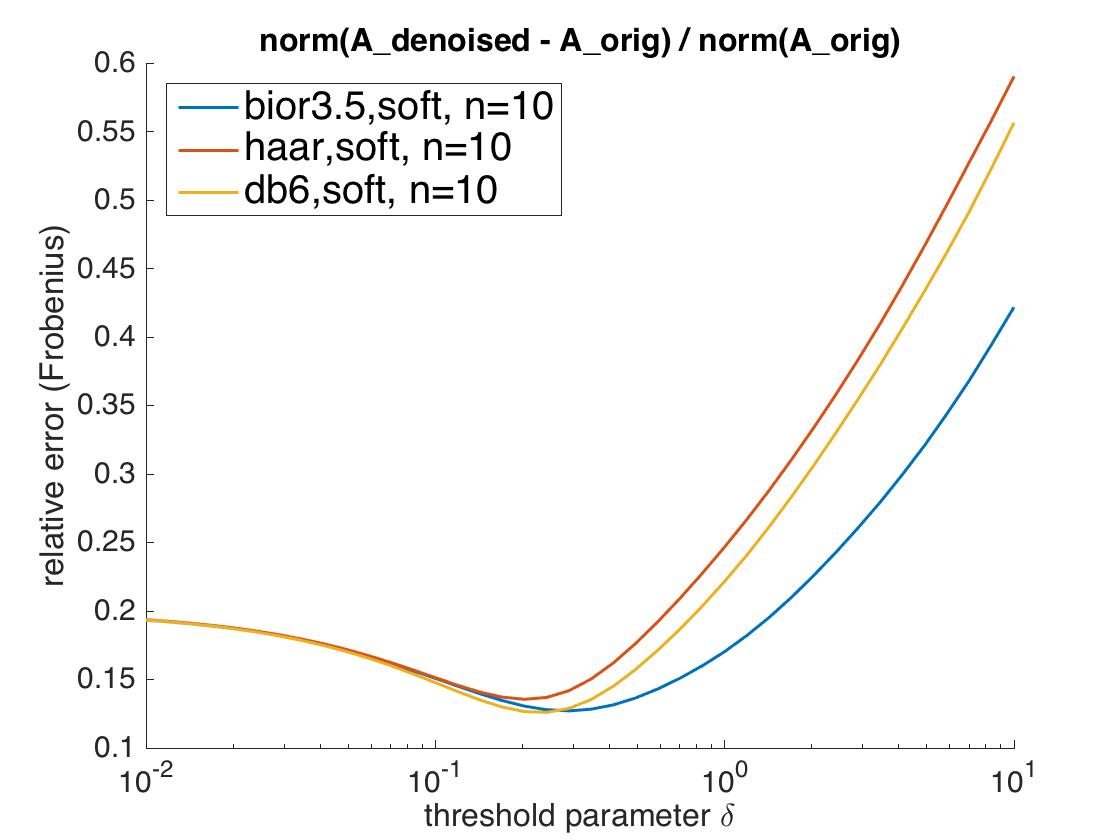
\includegraphics[width=\textwidth]{../src/denoising/denoised_err_wavekinds}
        \caption{Voor verschillende waarden van de threshold parameter $\delta$ is een noisy figuur gedenoised. De relatieve fout t.o.v. de originele figuur(zonder noise) is telkens berekent. De onbewerkte noisy figuur heeft een relatieve fout van $0.2$.verschillende soorten wavelets zijn gebruikt. Conclusie: opletten met de waarde van de threshold parameter..}
        \label{fig:mouse}
    \end{subfigure}
    \caption{plots error vs $\delta$}\label{fig:baboon}
\end{figure}

\end{document}
